%Copyright (c) 2004 2005 2006 Atos Origin
%Permission is granted to copy, distribute and/or modify this
%document
%under the terms of the GNU Free Documentation License,
%      Version 1.2
%      or any later version published by the Free Software
%      Foundation;
%      with no Invariant Sections, no Front-Cover
%      Texts, and no Back-Cover
%      Texts.  A copy of the license is
%      included in the section entitled "GNU
%      Free Documentation License".
%
%$Id: qualify.tex,v 1.1 2006/02/16 16:33:33 goneri Exp $
\section{Qualify}
\begin{figure}[h]
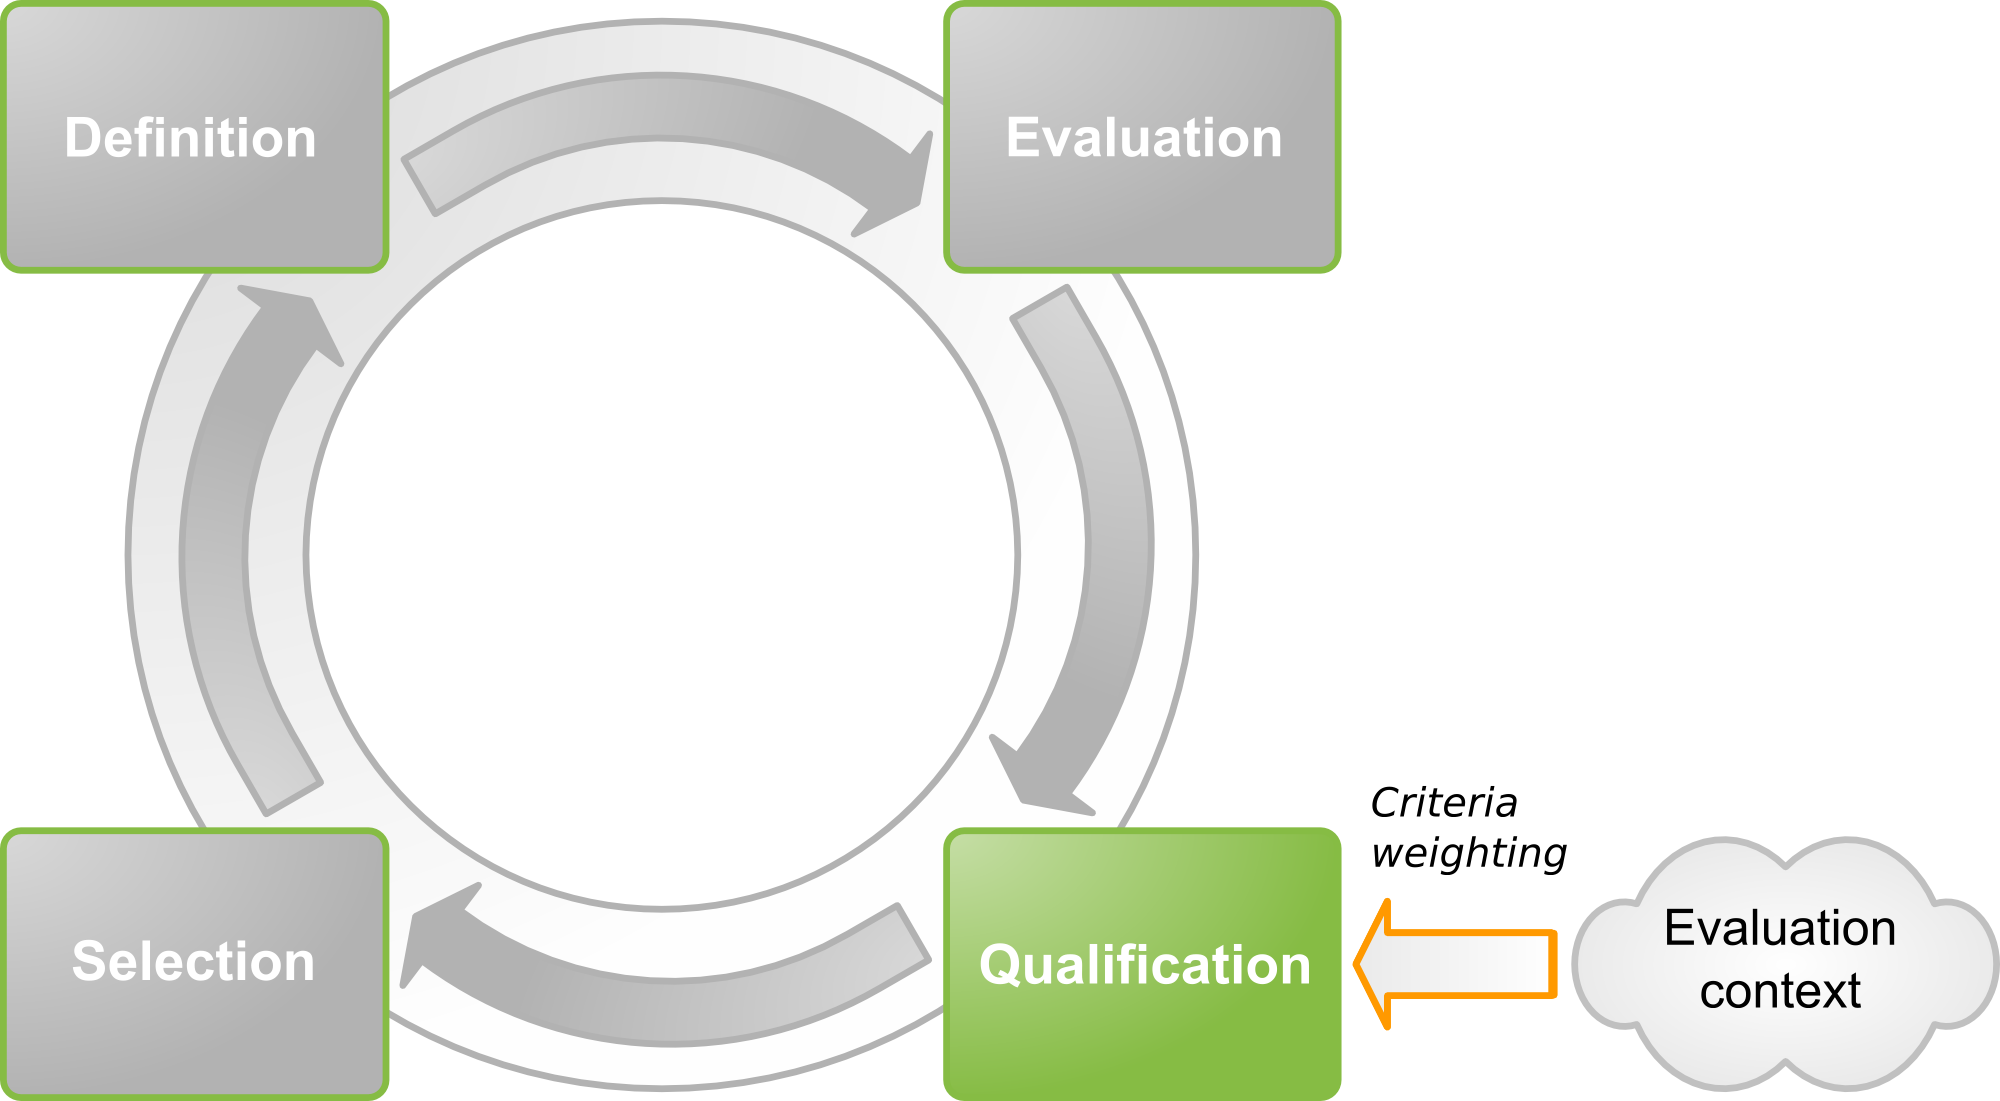
\includegraphics[width=13cm]{images/qualifier}
\caption{Step 3 - Qualify}
\end{figure}

\subsection{Objective}
The objective of this step is to define filters translating the needs and constraints 
related to the selection of a free or open source software in a specific context. 
This is achieved by qualifying the user's context which will be used later in Step - 4 "Select".


\subsection{Filter on ID card}
A first level of filtering can be defined on data from the software's ID card.


For instance, it could be to only consider software from a given family or 
compatible with a given operating system.


In general, although it is not mandatory, this filter does not include 
any weighting; it is mostly used to eliminate inadequate software 
in the specific context of the user.

\subsection{Filter on Functional grig}
Each functionality of the functional grid is attributed a requirement 
level selected among the following:

\begin{itemize}
\item required functionality
\item optional functionality
\item not required functionality
\end{itemize}

These requirement levels will be linked to weighting values at Step 4 - "Select", 
according to the selected mode of selection.

\subsection{Filter on User's risks}
The relevance of each criterion of this axis is positioned according to user's 
context, as indicated in figure~\ref{fig-relevance}.

\begin{figure}
\center
\begin{tabular}{|c|}
\hline \TS{Relevance}\\
\hline Irrelevant criterion, excluded from filter\\
\hline Relevant criterion\\
\hline Critical criterion\\
\hline
\end{tabular}
\label{fig-relevance}
\end{figure}
This relevance will be converted into a numerical weighting value at the following step, 
according to the selected mode of selection.

\subsection {Filter on Service provider's risks}
This filter is used by a service provider to evaluate software and services to be integrated in its offer and to determine the associated levels of commitment.


\subsection {O3S tool}
The O3S tool allows to define these different filters, while being guided with data entry.